\graphicspath{ {./figuresSimulation} }
\section{Simulation}
\subsection{Création du modèle}
Pour simuler notre dipôle nous utiliserons Flux2D d'Altair. La simulation se fait par élément fini. Cela consiste à dessiner notre géométrie pour la diviser en plusieurs points grâce à un maillage. Le logiciel résout en chaque point une équation différentielle dérivée des équations de Maxwell pour une application donnée. Pour mesurer une capacité nous simulerons dans le domaine de l'électrostatique. Nous nous intéresserons aux charges et aux champs électrique.

\subsubsection{Géométrie}
Flux nous permet de faire du dessin paramétrique. Nous pourrons ainsi, pendant la simulation, faire varier nos paramètres géométriques. Nous créons des paramètres pour toutes nos grandeurs: épaisseur et largeur. La profondeur est entrée à la création du modèle. Le logiciel intègre le fait que nous dessinons une coupe et utilisera la profondeur  pour les calcul qui concerne l'ensemble du système comme par exemple l'énergie total. Nous utilisons les valeurs défini pendant la conception, figure \ref{plan} et \ref{plancoupe}. Dans l’intérêt de la simulation nous ajoutons une couche d'eau. Nous ne pouvons pas simuler une goutte en deux dimensions. Nous étudierons un cas sans eau notre 0\% et un cas avec une couche continue notre 100\%. 

Le nombre de piste ne peut pas être paramétrisé car il crée des surfaces supplémentaires, ce qui n'est pas géré en simulation par Flux2D. Nous créerons trois projets pour trois nombre de piste: 20,10,5. Puisque la largeur du circuit et le nombre de pistes est fixe la somme distance et largeur de piste sera fixe aussi. Elle vaudra $S_{piste} = \frac{L_{pcb}}{N_{piste}}$. Si nous changeons la largeur des pistes nous devrons changer la distance. Nous utilisons alors un seul paramètre qui fera varier les deux. Il représente le rapport entre largeur et distance $F_{dist,larg} = \frac{L_{piste}}{D_{piste}} $. Nous pouvons définir largeur et distance en fonction de nos deux nouveaux paramètres: $D_{piste} = \frac{S_{piste}}{F_{dist,larg}+1}$, $L_{piste} = S_{piste} - \frac{S_{piste}}{F_{dist,larg}+1}$. C'est ces deux expressions que nous insérons dans le logiciel. 
Une fois tous les paramètres rentrés, nous construisons avec ceux-ci toute notre géométrie. On crée d'abord les points, puis on les relie pour former les lignes qui formerons nos surfaces. 

\begin{table}[!ht]
\begin{center}
\begin{tabular}{|l|l|}
\hline
Paramètre & valeur [mm]\\
\hline
EP\_CIBLE & 2.7\\
\hline
EP\_CUIVRE & 0.018\\
\hline
EP\_MASQUE & 0.035\\
\hline
EP\_PCB & 1.55\\
\hline
EP\_RESINE & 0.5\\
\hline
LARG\_PCB & 60\\
\hline
NBR\_PISTE & 20,10.5\\
\hline
FACTOR\_DIST\_LARG\_PISTE & variable\\
\hline
SUM\_DIST\_LARG\_PISTE & LARG\_PCB/NBR\_PISTE\\
\hline
LARG\_PISTE & {\tiny SUM\_DIST\_LARG\_PISTE-(SUM\_DIST\_LARG\_PISTE/(FACTOR\_DIST\_LARG\_PISTE+1))}\\
\hline
DIST\_PISTE & {\tiny SUM\_DIST\_LARG\_PISTE/(FACTOR\_DIST\_LARG\_PISTE+1)}\\
\hline
\end{tabular}
\caption{Liste des paramètre}
\end{center}
\end{table}

\begin{figure}[!ht]
 \centering
 \includegraphics[width=14cm]{c20geotout.png}
 \caption{Géométrie du modèle entier}
\end{figure}

\begin{figure}[!ht]
 \centering
 \includegraphics[width=14cm]{c20geozoom.png}
 \caption{Géométrie du modèle, zoom sur les pistes}
\end{figure}

\begin{description}
 \item[Bleu Foncé:] couche cible (eau)
 \item[Noir:] Résine
 \item[Vert:] Masque de soudure
 \item[Rouge:] Piste pôle 1
 \item[Bleu claire:] Piste pôle 2
 \item[Brun:] PCB
 \item[Turquoise:] Plan cuivre
\end{description}

Une dernière surface devra être créée pour représenter l'infini. Flux2d fonctionne en appliquant des conditions aux limite sur une sphère défini par l'utilisateur entourant notre modèle. Ces conditions permettent de simuler un environnement infini dans un zone fini. 

\subsubsection{Physique}
Une fois la géométrie terminée nous pouvons ajouter des contraintes physiques à notre modèle. Cela consiste à assigner des matériaux à nos surfaces. La résine, le masque et le pcb sont des isolants avec une certaine constante diélectrique. Le cuivre sera considéré comme un conducteur parfait. Une tension sera appliquée sur les deux pôles. Nous fixerons une tension de 3.3V et une autre de 1.65V. Cela nous donnera une différence de 1.65V. Nous l’enregistrerons dans un paramètre physique qui pourra être utilisé plus tard dans les calculs. Le plan de cuivre restera flottant. L'eau sera aussi considéré comme un isolant avec une constante diélectrique. La cible, le plan et la résine pourra être remplacé par de l'air au besoin de la simulation.


\begin{table}[!ht]
 \begin{center}
\begin{tabular}{|l|l|l|l|}
\hline
Surface & Matériau & $\mu_r$ & Potentiel\\
\hline
Cible & eau & 80 & -\\
\hline
Résine & résine & 4 & -\\
\hline
Masque & résine & 4 & -\\
\hline
Piste P1 & conducteur parfait & - & 3.3 V\\
\hline
Piste P2 & conducteur parfait & - & 1.65 V\\
\hline
PCB & FR4 & 4.4 & -\\
\hline
Plan & conducteur parfait & - & flotant\\
\hline
\end{tabular}
\caption{Caractéristiques physique}
\end{center}
\end{table}



\subsubsection{Maillage}
Le maillage est une partie importante de la création d'un modèle du simulation par élément fini. Un compromis doit être trouvé entre le temps de calcul et la résolution de la simulation. Quelques règles assez simple permettent d'obtenir des résultats convenables. Plus le champs est intense à un endroit plus le maillage doit être fin. Il faut aussi être fin aux intersections entre deux matières. Les grandes surfaces peuvent être plus relâchées aux centre. En suivant ces recommandations, nous obtenons un maillage satisfaisant.


\begin{figure}[!ht]
 \centering
 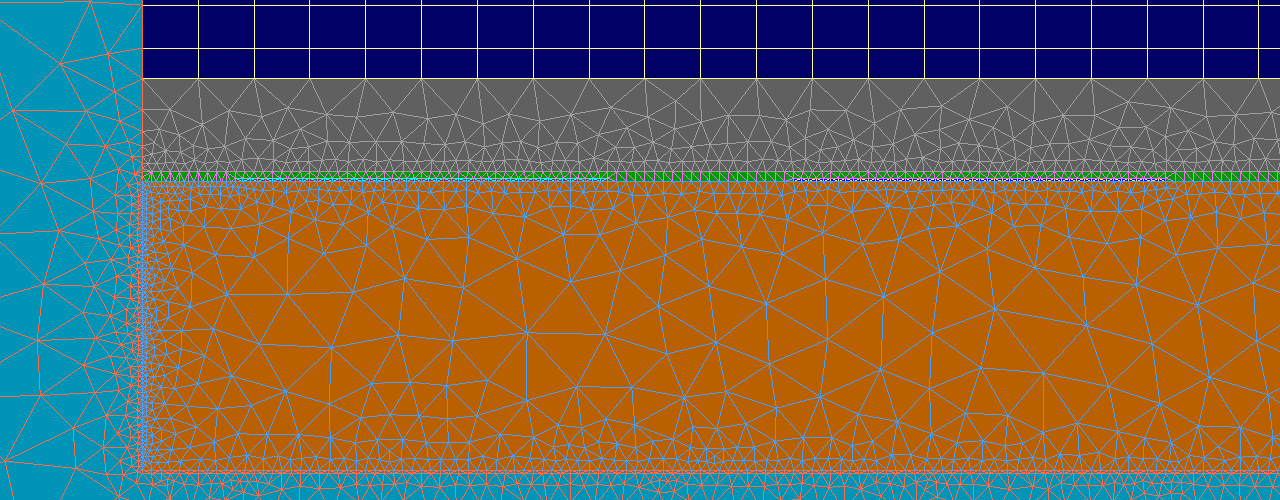
\includegraphics[width=14cm]{C20maillage.png}
 \caption{Maillage du modèle}
\end{figure}


\subsection{Exploitation}

\subsubsection{20 pistes}
Nous pouvons à présent démarrer les simulations. Nous commencerons avec 20 pistes et un rapport entre largeur et distance de 2 (largeur des pistes = 2mm, distance entre piste = 1mm). La cible ainsi que le plan seront en air. Une fois la simulation terminée, nous pouvons afficher le champs magnétique ainsi que les lignes du potentiel électrique pour analyser le résultat et vérifier que la simulation s'est bien passé.

\begin{figure}[!ht]
 \centering
 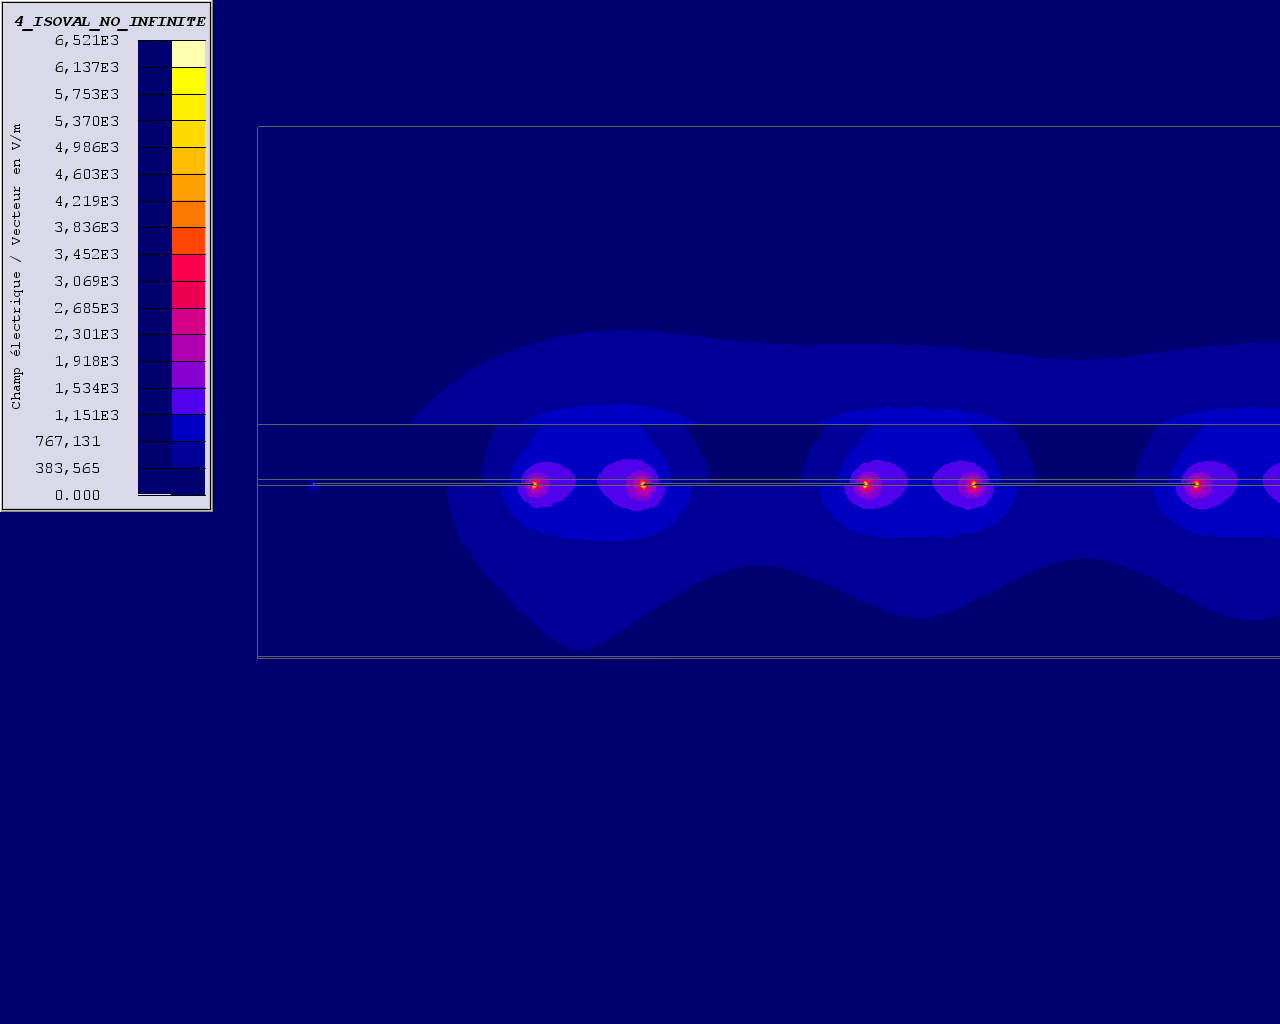
\includegraphics[width=14cm]{simulationChampElectrique.png}
 \caption{Champs électrique 20 pistes}
\end{figure}

\newpage
\begin{figure}[!ht]
 \centering
 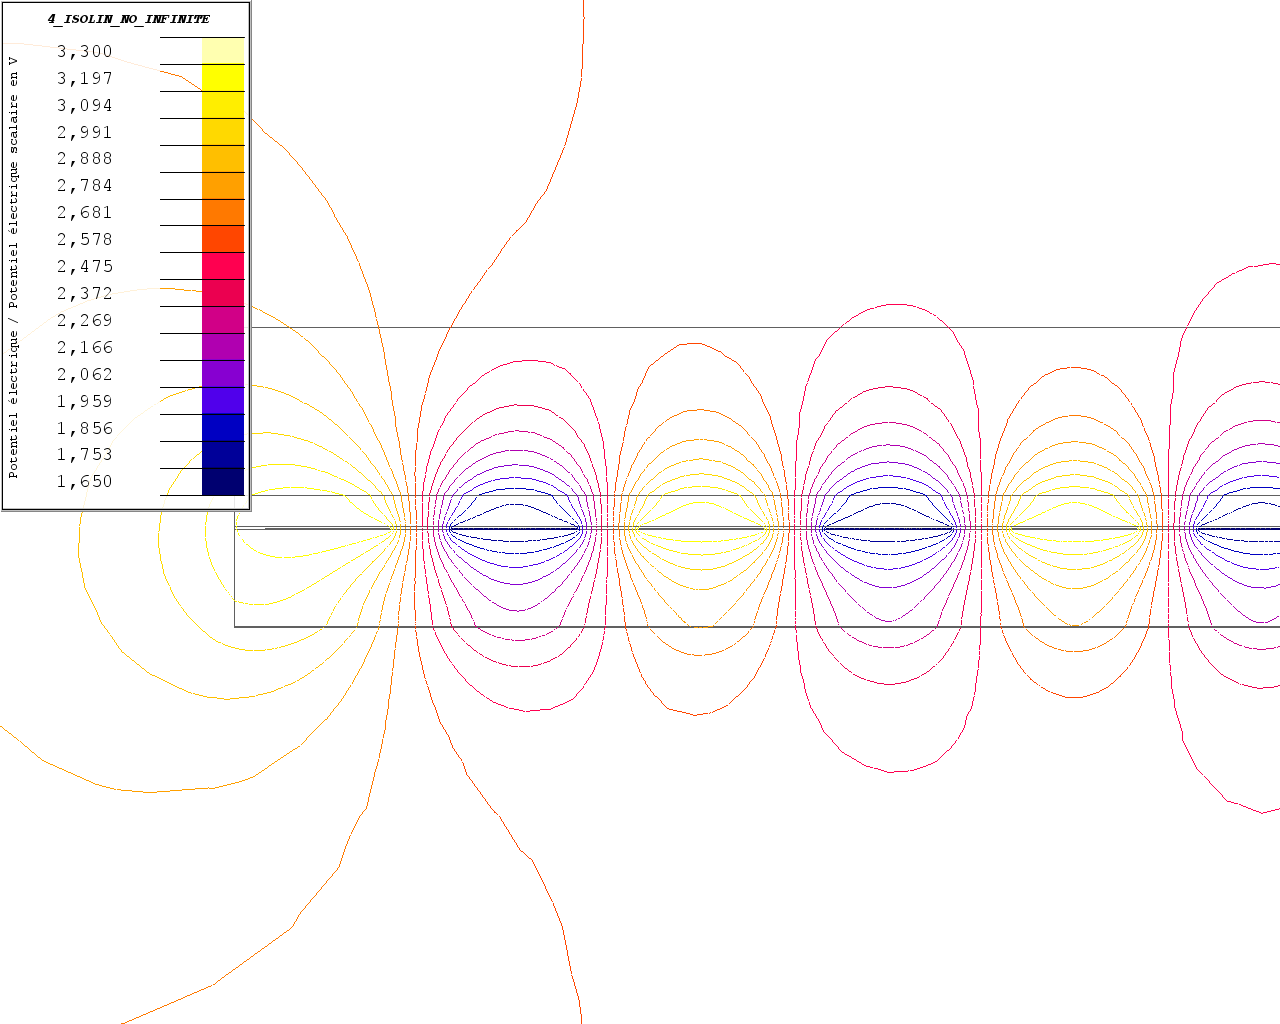
\includegraphics[width=14cm]{C20air.png}
 \caption{Lignes de potentiel électrique 20 pistes}
\end{figure}

On remarque premièrement sur ces graphiques que le maillage est correct. Les lignes sont bien continue même très proche des conducteurs. Les coupures des niveaux du champs magnétique sont dues à la transition d'un milieu à un autre et sont tout à fait normal. La deuxième information que nous fournit ces figures sont le fait que le champs est bien présent dans l'espace de la cible. Cela veut dire qu'un changement de caractéristique à ce niveau aura une influence sur le champs et donc la capacité. C'est positif pour la viabilité de notre capteur.

Nous pouvons calculer dans cette simulation la capacité de notre système. Nous utilisons pour cela la définition de la capacité qui dépend de l'énergie $C = \frac{2W}{U^2}$. Flux2d intègre tout les points pour calculer l'énergie électrique de tous le modèle en prenant en compte la profondeur spécifiée ultérieurement. Nous utilisons la tension que nous avions mis en paramètre pour attribuer l’expression de la capacité dans un paramètre qu'on appellera C\_total. Ce paramètre sera disponible pour nos prochaine simulation afin d'obtenir directement la valeur et tracer des graphiques. Pour cette première simulation C vaut \SI{78.98}{\pico\farad}. Nous somme au dessus de l'offset maximal de notre convertisseur qui est de 10pF. Nous somme cependant dans le bonne ordre de grandeurs et il ne sera pas difficile de diminuer la capacité. 

Nous pouvons jouer avec le rapport distance et largeur de piste afin d'observer comment la capacité varie. Nous créons pour cela un scénario de simulation pour faire varier notre paramètre de 0.5 à 2 sur 10 pas. On remarque bien une diminution de la capacité mais ce n'est pas suffisant. Nous observerons plus tard comment elle diminue encore en réduisant le nombre de piste.

\newpage

\begin{figure}[!ht]
 \centering
 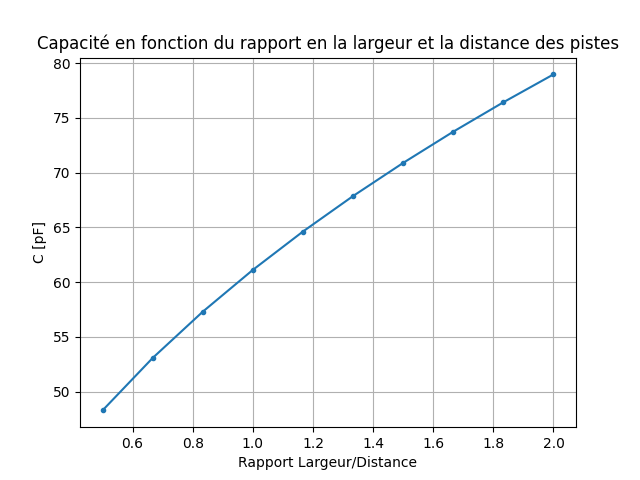
\includegraphics[width=10cm]{C20airGraph.png}
 \caption{Capacité en fonction du rapport distance/largeur}
\end{figure}

Nous allons à présent changer la cible en eau afin d'observer les changements produits.


\begin{figure}[!ht]
 \centering
 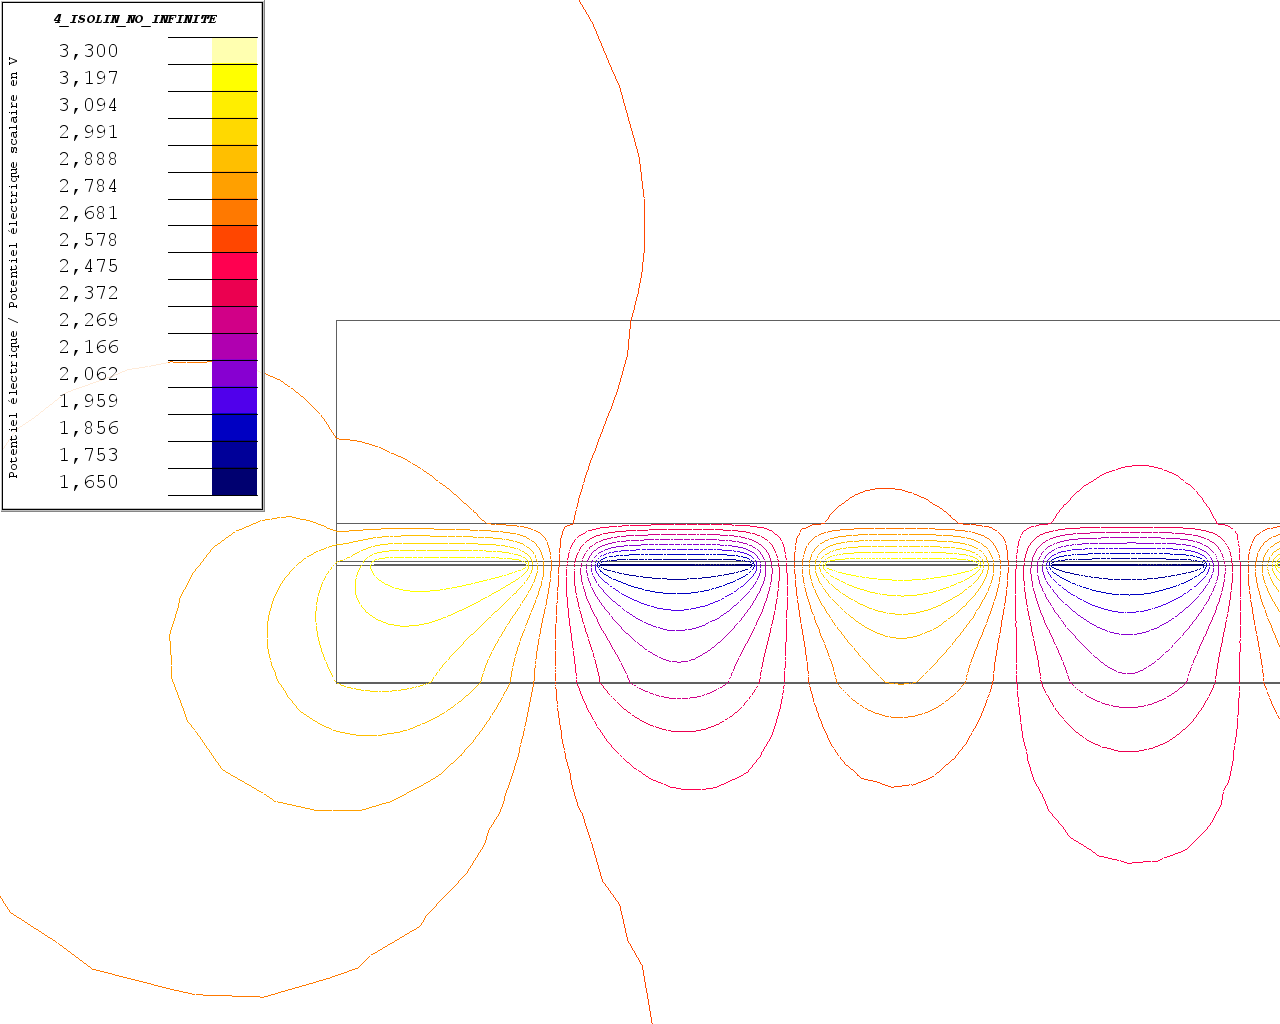
\includegraphics[width=14cm]{C20eauligne.png}
 \caption{Lignes de potentiel électrique 20 pistes avec eau}
 \label{c20eaul}
\end{figure}

\begin{figure}[!ht]
 \centering
 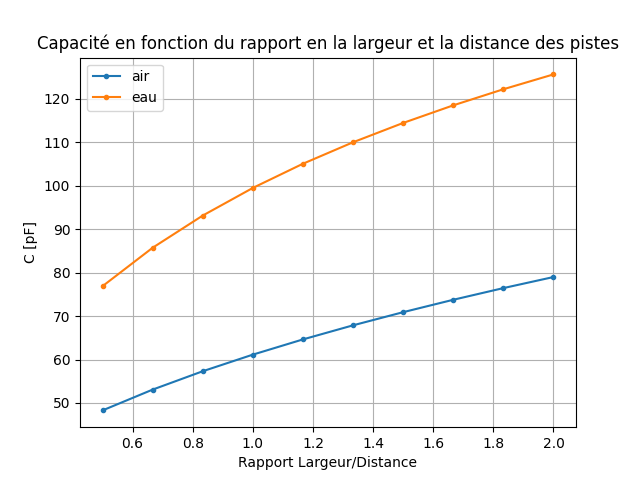
\includegraphics[width=7cm]{C20eauGraph1.png}
 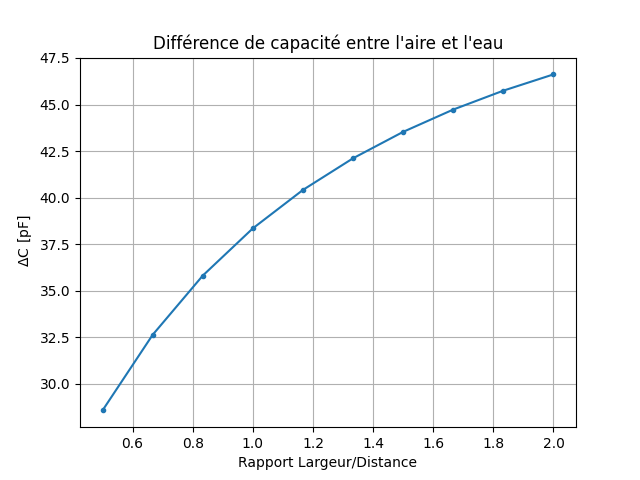
\includegraphics[width=7cm]{C20eauGraph2.png}
 \caption{Comparaison des capacité avec et sans eau pour 20 pistes}
\end{figure}

L'eau modifie bien le champs électrique. On vois sur la figure \ref{c20eaul} que le champs est comprimé. L'effet de l'eau sur la capacité est tout aussi visible. La capacité augmente de près de la moitié de sa valeur. Un fait intéressent est que la différence évolue plus vite que l'offset de capacité. Cela veut dire que si on diminue trop le rapport pour faire diminuer la capacité d'offset on risque de réduire beaucoup trop la sensibilité, bien que nous somme toujours au dessus du seuil de notre convertisseur.

\subsubsection{5 et 10 pistes}
Nous effectuons une simulation avec 5 et 10 piste sur la carte. Nous utilisons toujours le même scénario avec et sans eau.


\begin{figure}[!ht]
 \centering
 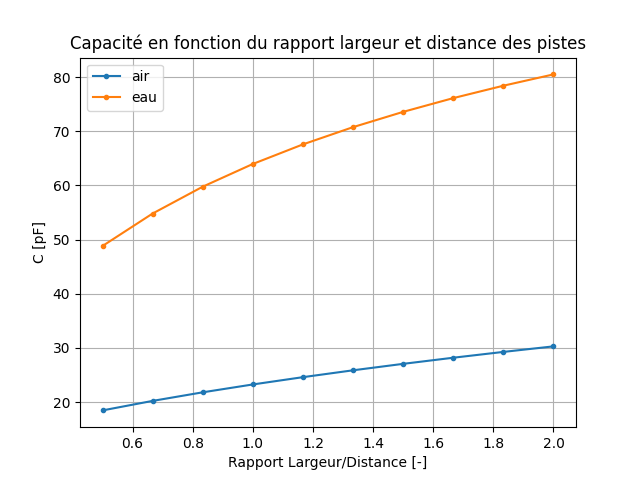
\includegraphics[width=7cm]{C10Graph1.png}
 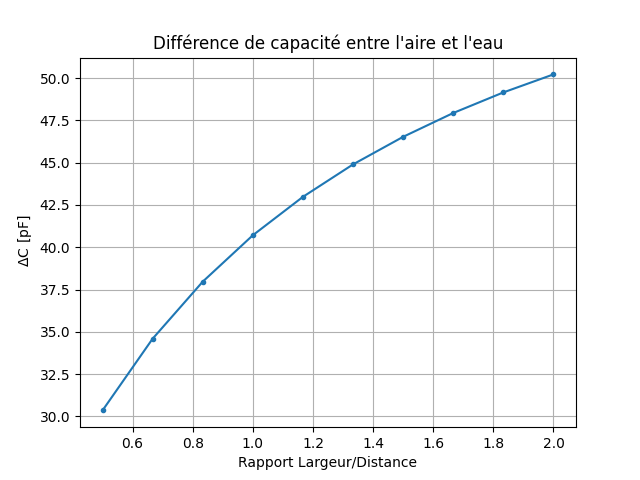
\includegraphics[width=7cm]{C10Graph2.png}
 \caption{Comparaison des capacité avec et sans eau pour 10 pistes}
\end{figure}

Cette nouvelle configuration est meilleur que la première. la capacité d'offset a été divisé par deux tout en gardant un bon delta. Nous somme à présent plus proche des caractéristiques du convertisseur.

\begin{figure}[!ht]
 \centering
 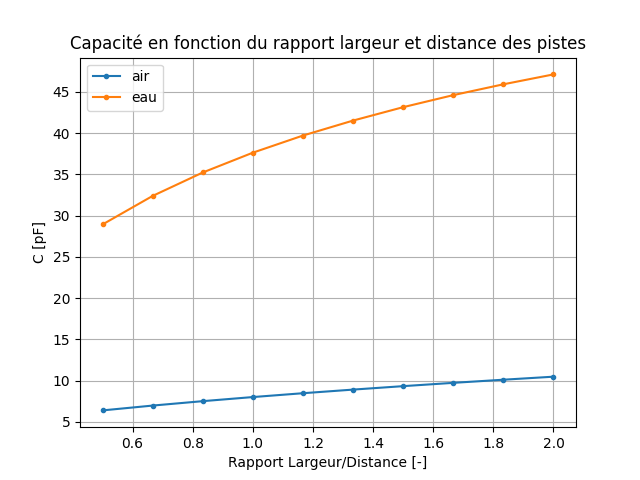
\includegraphics[width=7cm]{C5Graph1.png}
 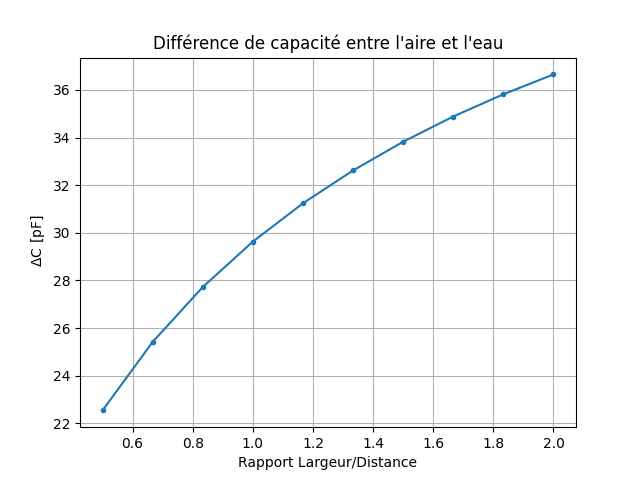
\includegraphics[width=7cm]{C5Graph2.png}
 \caption{Comparaison des capacité avec et sans eau pour 5 pistes}
\end{figure}
\newpage

Grâce à 5 piste nous atteignons enfin la capacité d'offset cherchée. La différence de capacité a diminué mais est toujours très élevée si on la compare à l'offset. Ces résultats sont à bien considérer car le modèle ne nous permet pas de simuler de fine goutte entre les lignes. Il est donc difficile de prévoir si une carte avec moins de ligne peut capter toutes les gouttes. Seules les mesures permettrons de nous le dire. 

\subsubsection{Plan de cuivre}

L'utilisation d'un plan de cuivre a été pensé pour concentrer la mesure à la surface haute de la carte. Nous appliqueront donc un conducteur parfait à la couche sous le pcb. Nous allons dans un premier temps simuler l'effet d'un plan seulement sur le modèle à 5 lignes pour comprendre son effet. Nous lancerons le même scénario avec et sans eau pour que nous puissions comparer.

\begin{figure}[!ht]
 \centering
 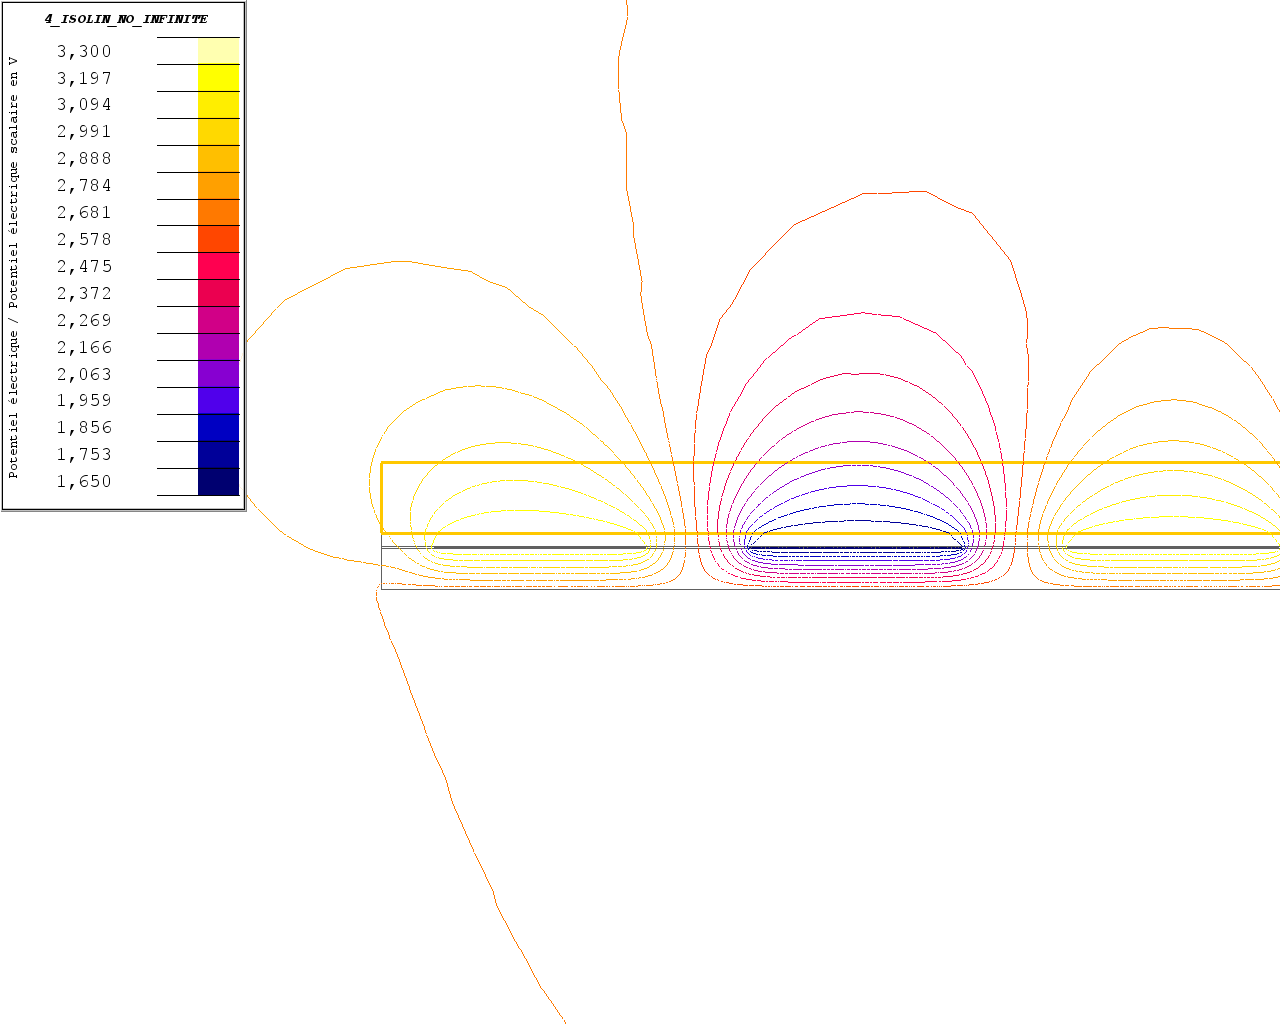
\includegraphics[width=10cm]{C5airMasseligne.png}
 \caption{Lignes de potentiel électrique, avec plan, avec eau pour 5 pistes}
 \label{c5planlair}
\end{figure}

\begin{figure}[!ht]
 \centering
 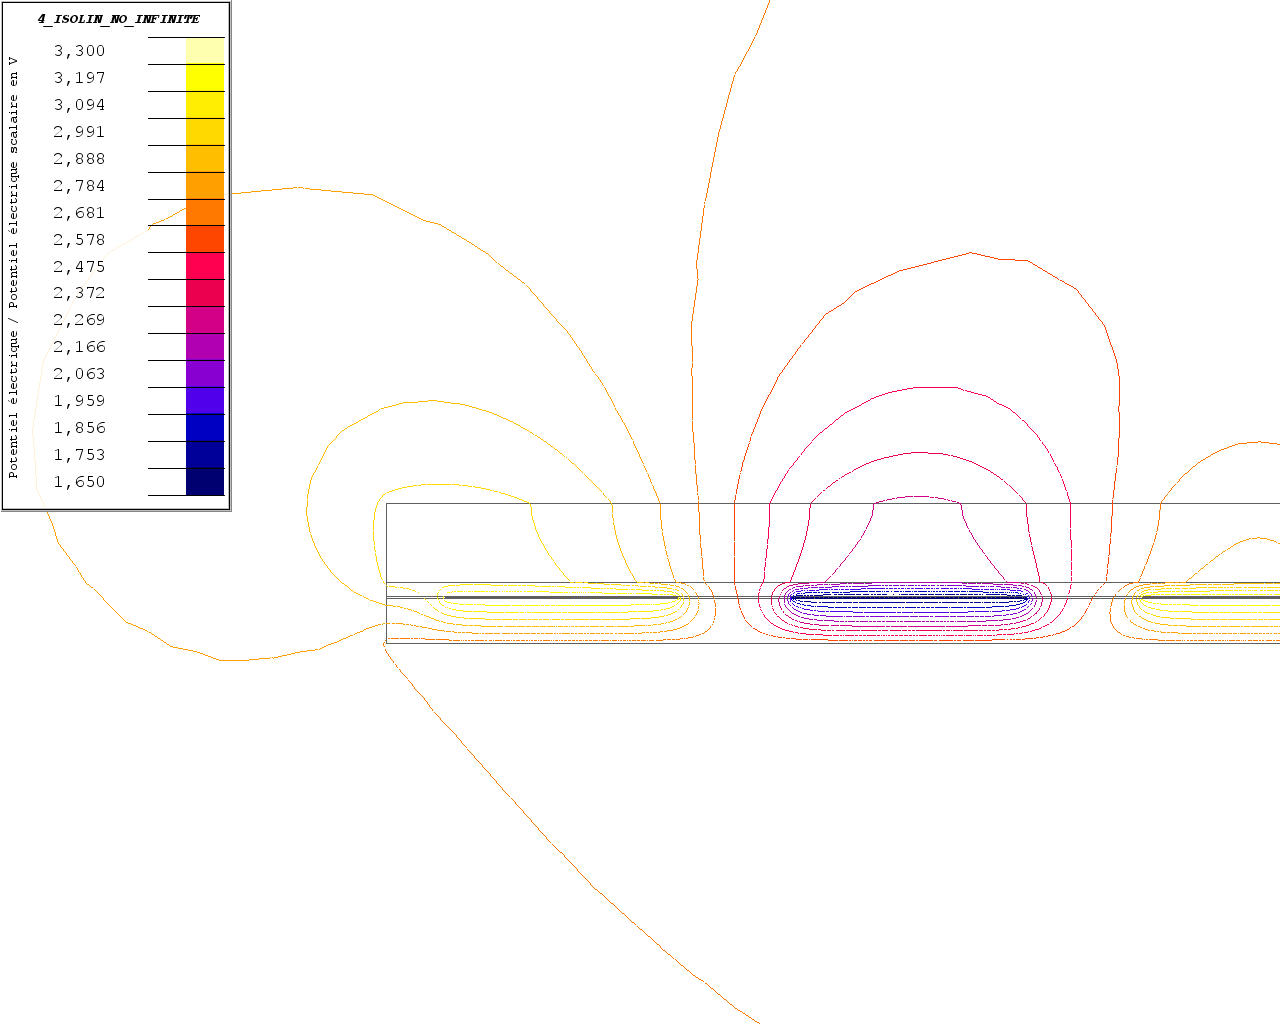
\includegraphics[width=10cm]{C5eauMasseligne.png}
 \caption{Lignes de potentiel électrique, avec plan, sans eau pour 5 pistes}
 \label{c5planleau}
\end{figure}

\newpage

\begin{figure}[!ht]
 \centering
 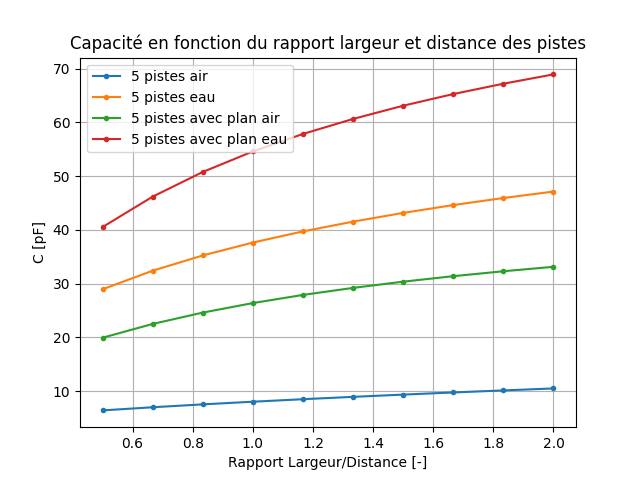
\includegraphics[width=7cm]{C5masseGraph1.png}
 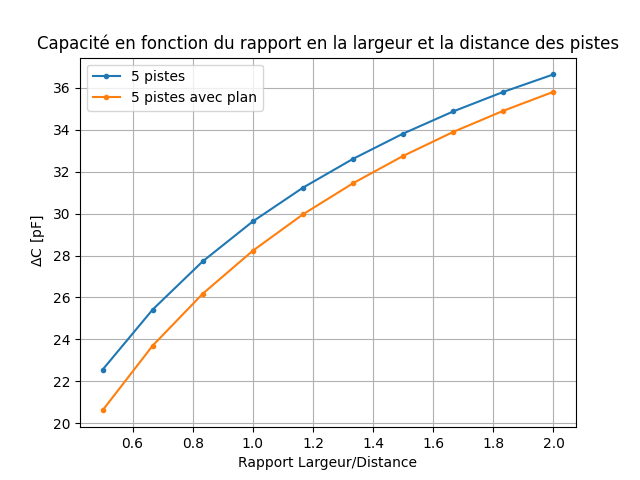
\includegraphics[width=7cm]{C5masseGraph2.png}
 \caption{Comparaison des capacité, avec plan, avec et sans eau pour 5 pistes}
\end{figure}

L'ajout d'un plan augmente l'offset et diminue le delta ce qui n'est pas très intéressant pour nous. Cependant on voit sur la figure \ref{c5planlair} et \ref{c5planleau} que les lignes de potentiel ne sortent plus par dessous. On en déduit grâce au graphique que, comme prévu, tout ce qui se passe en dessous n’influencera plus notre capteur. Nous garderons cette configuration pour nos mesures. Afin d'obtenir des valeur de comparaison pour les mesures nous effectuons une dernière simulation avec le plan de cuivre pour 10 et 20 pistes. 

\begin{figure}[!ht]
 \centering
 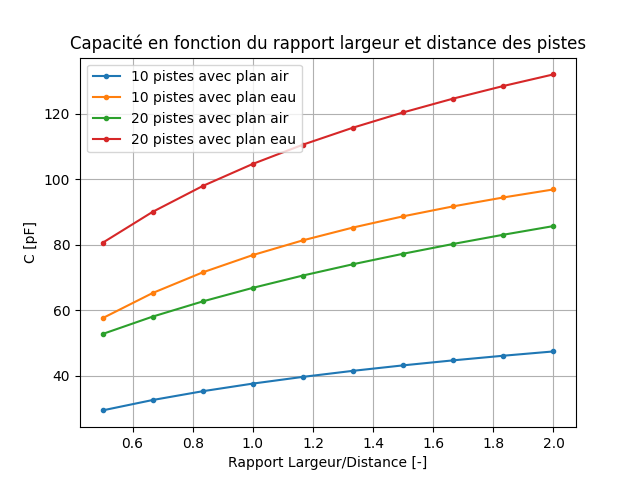
\includegraphics[width=7cm]{C1020masseGraph1.png}
 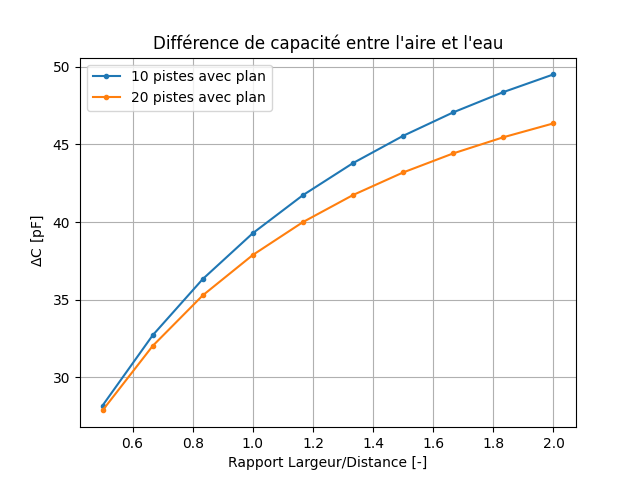
\includegraphics[width=7cm]{C1020masseGraph2.png}
 \caption{Capacité, avec plan, avec et sans eau pour 10 et 20 pistes}
\end{figure}

Encore une fois, les performances avec 10 pistes sont meilleures qu'avec 20 piste. Avec le plan de cuivre, la configuration de 10 piste a toujours un plus faible offset et une plus grande sensibilité. Pour cette raison, nous n'utiliserons pas de 20 pistes pour la suite.
